%package list
\documentclass{article}
\usepackage[top=3cm, bottom=3cm, outer=3cm, inner=3cm]{geometry}
\usepackage{graphicx}
\usepackage{url}
%\usepackage{cite}
\usepackage{hyperref}
\usepackage{array}
%\usepackage{multicol}
\newcolumntype{x}[1]{>{\centering\arraybackslash\hspace{0pt}}p{#1}}
\usepackage{natbib}
\usepackage{pdfpages}
\usepackage{multirow}
\usepackage{multirow}
\usepackage[T1]{fontenc}
\usepackage{imakeidx}
% Imagenes de costado
\usepackage{wrapfig}
\usepackage{graphicx}

% Modificar URLs
\usepackage{hyperref}
\hypersetup{
    colorlinks=true,
    linkcolor=black,
    filecolor=magenta,      
    urlcolor=blue,
    pdftitle={Overleaf Example},
    pdfpagemode=FullScreen,
    }

\urlstyle{same}


\usepackage[normalem]{ulem}
\useunder{\uline}{\ul}{}

\usepackage{minted}

% codigo fuente
\usepackage{listings}
\usepackage{color, colortbl}
\definecolor{dkgreen}{rgb}{0,0.6,0}
\definecolor{gray}{rgb}{0.5,0.5,0.5}
\definecolor{mauve}{rgb}{0.58,0,0.82}
\definecolor{codebackground}{rgb}{0.95, 0.95, 0.92}
\definecolor{tablebackground}{rgb}{0.0, 0.45, 0.63}
\lstset{frame=tb,
	language=bash,
	aboveskip=3mm,
	belowskip=3mm,
	showstringspaces=false,
	columns=flexible,
	basicstyle={\small\ttfamily},
	numbers=none,
	numberstyle=\tiny\color{gray},
	keywordstyle=\color{blue},
	commentstyle=\color{dkgreen},
	stringstyle=\color{mauve},
	breaklines=true,
	breakatwhitespace=true,
	tabsize=3,
	backgroundcolor= \color{codebackground},
}

%%%%%%%%%%%%%%%%%%%%%%%%%%%%%%%%%%%%%%%%%%%%%%%%%%%%%%%%%%%%%%%%%%%%%%%%%%%%
%%%%%%%%%%%%%%%%%%%%%%%%%%%%%%%%%%%%%%%%%%%%%%%%%%%%%%%%%%%%%%%%%%%%%%%%%%%%
\newcommand{\csemail}{vmachacaa@ulasalle.edu.pe}
\newcommand{\csdocente}{MSc. Maribel Molina Barriga}
\newcommand{\cscurso}{Sistemas Operativos}
\newcommand{\csuniversidad}{Universidad La Salle}
\newcommand{\csescuela}{Escuela Profesional de Ingeniería de Software}
\newcommand{\cspracnr}{02}
\newcommand{\cstema}{Comandos en Windows y Linux}
%%%%%%%%%%%%%%%%%%%%%%%%%%%%%%%%%%%%%%%%%%%%%%%%%%%%%%%%%%%%%%%%%%%%%%%%%%%%
%%%%%%%%%%%%%%%%%%%%%%%%%%%%%%%%%%%%%%%%%%%%%%%%%%%%%%%%%%%%%%%%%%%%%%%%%%%%


\usepackage[english,spanish]{babel}
\usepackage[utf8]{inputenc}
\AtBeginDocument{\selectlanguage{spanish}}
\renewcommand{\figurename}{Figura}
\renewcommand{\refname}{Referencias}
\renewcommand{\tablename}{Tabla} %esto no funciona cuando se usa babel
\AtBeginDocument{%
	\renewcommand\tablename{Tabla}
}

\usepackage{fancyhdr}
\pagestyle{fancy}
\fancyhf{}
\setlength{\headheight}{30pt}
\renewcommand{\headrulewidth}{1pt}
\renewcommand{\footrulewidth}{1pt}
\fancyhead[L]{\raisebox{-0.2\height}{
\includegraphics[width=3cm]{logo_ulasalle (1).png}}}
\fancyhead[C]{}
\fancyhead[R]{\fontsize{7}{7}\selectfont	\csuniversidad \\ \csescuela \\ \textbf{\cscurso} }
\fancyfoot[L]{}
\fancyfoot[C]{Sistemas Operativos}
\fancyfoot[R]{Página \thepage}



\begin{document}

	\vspace*{10px}
	
	\begin{center}	
		\fontsize{17}{17} \textbf{ Práctica \cspracnr}
	\end{center}
	%\centerline{\textbf{\underline{\Large Título: Informe de revisión del estado del arte}}}
	%\vspace*{0.5cm}
	

\renewcommand{\arraystretch}{1.5}
\begin{table}[h]
	\begin{tabular}{|x{4.7cm}|x{4.8cm}|x{4.8cm}|}
		\hline 
		\textbf{DOCENTE} & \textbf{CARRERA}  & \textbf{CURSO}   \\
		\hline 
		\csdocente & \csescuela & \cscurso    \\
		\hline 
	\end{tabular}
\end{table}	

\begin{table}[h]
	\begin{tabular}{|x{4.7cm}|x{4.8cm}|x{4.8cm}|}
		\hline 
		\textbf{GRUPO} & \textbf{TEMA}  & \textbf{DURACIÓN}   \\
		\hline 
		\ 6 & \cstema & 5 horas   \\
		\hline 
	\end{tabular}
\end{table}
\renewcommand{\arraystretch}{1} 
	\section*{Integrantes}
	 	\begin{itemize}
                    \item José Carlos Machaca Vera
	 		\item Jhosep Alonso Mollapaza Morocco
	 		\item Patrick Andres Ramirez Santos
	 \end{itemize}
 
	\tableofcontents


	

\newpage

\section{Objetivos}
Se busca demostrar como la comprensión de los sistemas operativos a través de la ejecución práctica de comandos en Windows y Linux ayuda a mejorar la versatibilidad de los desarrolladores de software. Ademas se desea tener una guía pra manejar archivos y directorios, instalar programas y reconocer las diferencias al usar la terminal. 

\section{Software utilizado}
\begin{itemize}
    \item Overleaf
    \item Windows
        \begin{itemize}
            \item Windows 11
            \item Simbolo de Sistema
            \item Blog de notas
        \end{itemize}
    \item Linux
        \begin{itemize}
            \item Fedora 39
            \item Warp Terminal
            \item Neovim
        \end{itemize}
\end{itemize}

\newpage

\section{Windows}
    \subsection{Ejecutamos la consola}
        Se realiza mediante el cuadro de diálogo Ejecutar con la combinación de teclas Windows R y escribiendo cmd en este mismo.
    
    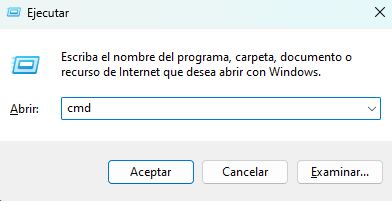
\includegraphics[scale=1.5]{WindowsCapturas/CuadroCMD.png}

    \subsection{Creamos carpeta LABSO}
        Una vez dentro del cmd, creamos la carpeta LABSO con el comando MD, una vez creada para ingresar a dicha carpeta es mediante el comando CD.
        \begin{minted}{bash}
        C:\Users\jhose>MD LABSO
        C:\Users\jhose>CD LABSO
        \end{minted}
        
        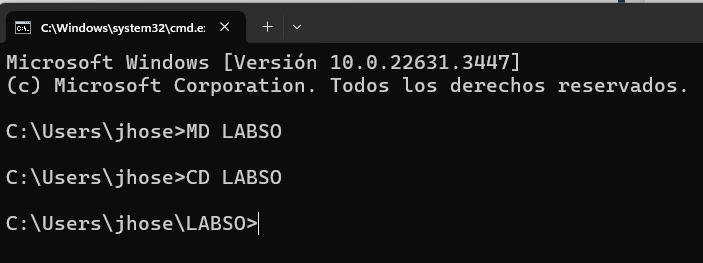
\includegraphics[scale=0.8]{WindowsCapturas/CreacionLABSO.png}  

    \subsection{Creamos directorios dentro de LABSO}
        Una vez creada la carpeta LABSO y dentro, creamos otras 2 carpetas, que son MEMORIA y PROCESOS, luego dentro de estas 2 carpetas creadas se crean otras 2 carpetas llamadas TEORIA y PRACTICA.
        \begin{minted}{bash}
        C:\Users\jhose\LABSO>MD MEMORIA PROCESOS
        C:\Users\jhose\LABSO>CD MEMORIA
        C:\Users\jhose\LABSO\MEMORIA>MD TEORIA PRACTICA
        C:\Users\jhose\LABSO\MEMORIA>CD..
        C:\Users\jhose\LABSO>CD PROCESOS
        C:\Users\jhose\LABSO\PROCESOS>MD TEORIA PRACTICA
        C:\Users\jhose\LABSO\PROCESOS>CD..
        \end{minted}
        
        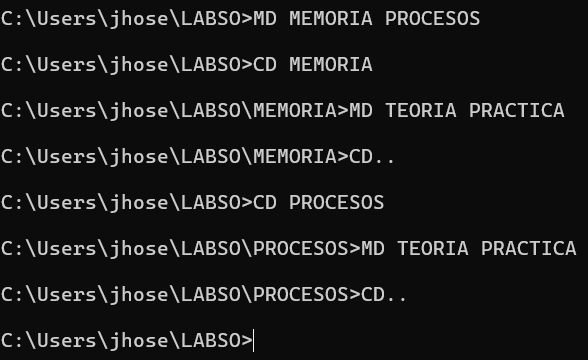
\includegraphics[scale=0.8]{WindowsCapturas/Carpetas.png}  

    \subsection{Usamos el comando TREE}
        Volvemos a la carpeta LABSO y ejecutamos el comando TREE para observar las carpetas que hay dentro de esta misma.
    
    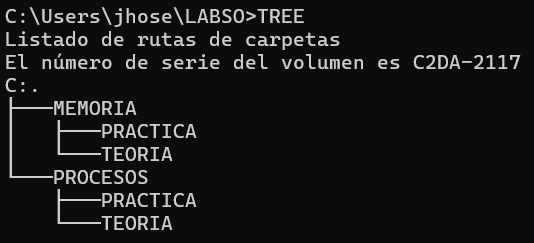
\includegraphics[scale=1]{WindowsCapturas/TREE.png}

    \subsection{Archivo .txt y comandos DIR, TYPE}
        Creamos un archivo .txt dentro de la carpeta MEMORIA.

    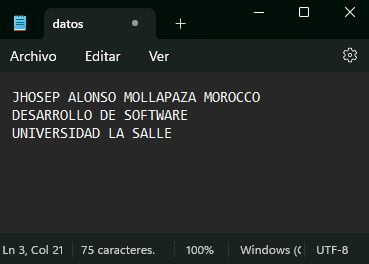
\includegraphics[scale=1.2]{WindowsCapturas/datostxt.png}  

        Luego usamos el comando DIR dentro de MEMORIA para listar los archivos y/o directorios.
        \begin{minted}{bash}
        C:\Users\jhose\LABSO>cd MEMORIA
        C:\Users\jhose\LABSO\MEMORIA>DIR
        \end{minted}
        
    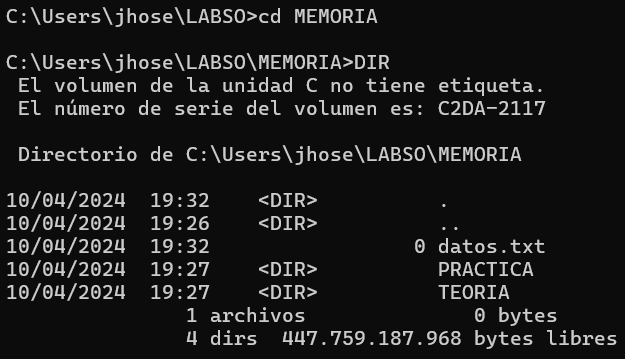
\includegraphics[scale=0.8]{WindowsCapturas/DirMemoria.png}  

        Y usamos el comando TYPE para observar el contenido del archivo datos.txt.
        \begin{minted}{bash}
        C:\Users\jhose\LABSO\MEMORIA>TYPE datos.txt
        JHOSEP ALONSO MOLLAPAZA MOROCCO
        DESARROLLO DE SOFTWARE
        UNIVERSIDAD LA SALLE
        \end{minted}
        
    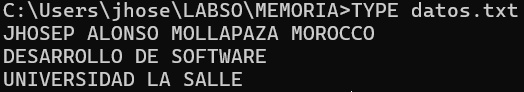
\includegraphics[scale=1]{WindowsCapturas/TypeDatos.png}

    \subsection{Copiar y renombrar datos.txt}
        Ahora se copiara el archivo datos.txt al directorio TEORIA dentro de PROCESOS, y una vez copiado iremos a esa carpeta para usar DIR y mostrar los archivos.
        \begin{minted}{bash}
        C:\Users\jhose\LABSO\MEMORIA>COPY datos.txt C:\Users\jhose\LABSO\PROCESOS\TEORIA
        C:\Users\jhose\LABSO\MEMORIA>CD..
        C:\Users\jhose\LABSO>CD PROCESOS
        C:\Users\jhose\LABSO\PROCESOS>CD TEORIA
        C:\Users\jhose\LABSO\PROCESOS\TEORIA>DIR
        \end{minted}
        
        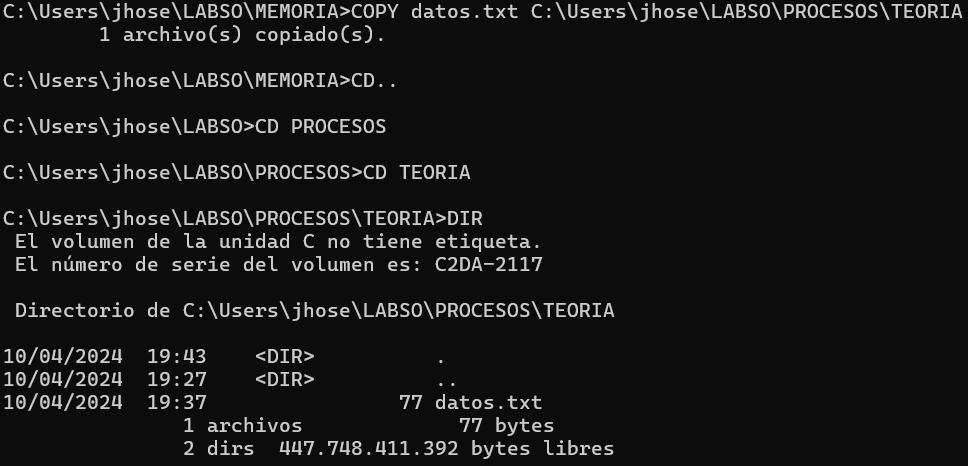
\includegraphics[scale=0.6]{WindowsCapturas/CopiarTXT.png}  

        Ahora cambiaremos el nombre de este archivo datos.txt por nombres.txt y lo verificaremos con el mismo comando DIR
        \begin{minted}{bash}
        C:\Users\jhose\LABSO\PROCESOS\TEORIA>REN datos.txt nombres.txt
        C:\Users\jhose\LABSO\PROCESOS\TEORIA>DIR
        \end{minted}

        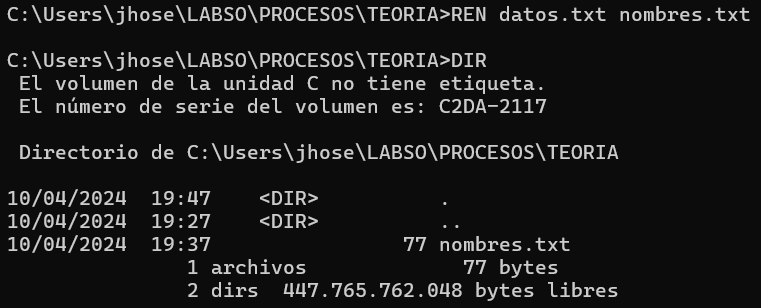
\includegraphics[scale=0.8]{WindowsCapturas/RenombrarTXT.png}  

    \subsection{Probando RD, DEL y diferentes parámetros de DIR}
        Se ha creado una carpeta llamada PRUEBA y un archivo PRUEBA.txt para probar los comandos RD y DEL que son para borrar carpetas y archivos respectivamente.
        \begin{minted}{bash}
        C:\Users\jhose\LABSO>DIR
        C:\Users\jhose\LABSO>RD PRUEBA
        C:\Users\jhose\LABSO>DEL PRUEBA.txt
        \end{minted}
        
        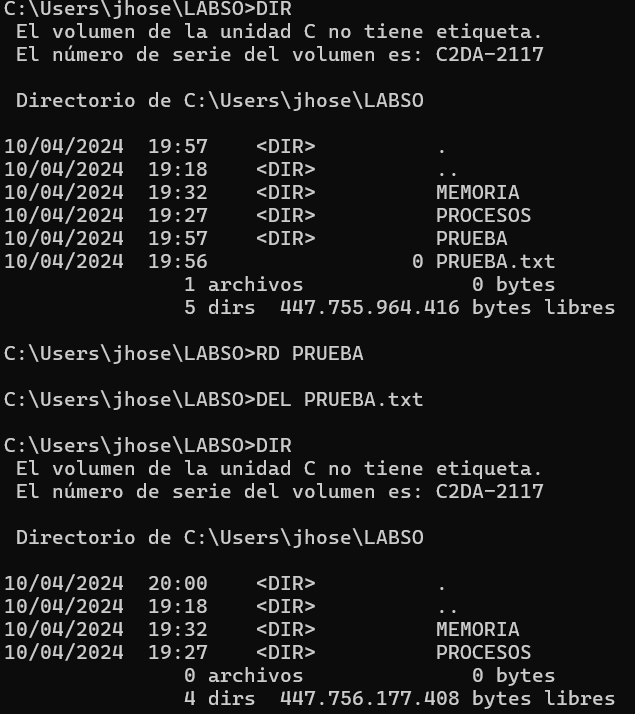
\includegraphics[scale=0.6]{WindowsCapturas/DELyRD.png}  

        Probando diferentes parámetros de DIR: \\ \\
        \begin{tabular}{cc}
        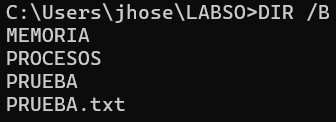
\includegraphics[width=.4\linewidth,valign=m]{WindowsCapturas/DIRB.png} & 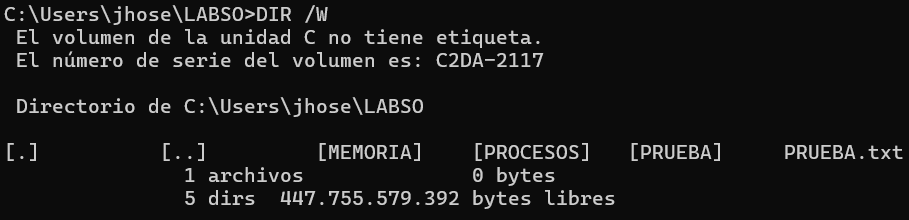
\includegraphics[width=.6\linewidth,valign=m]{WindowsCapturas/DIRW.png} \\
        DIR /B & DIR /W \\
    \end{tabular}

\section{Linux}

\subsection{Manipulando el shell}
Verificamos que la shell esté usando BASH con el siguiente comando:
        \begin{minted}{bash}
        echo $BASH
        \end{minted}
        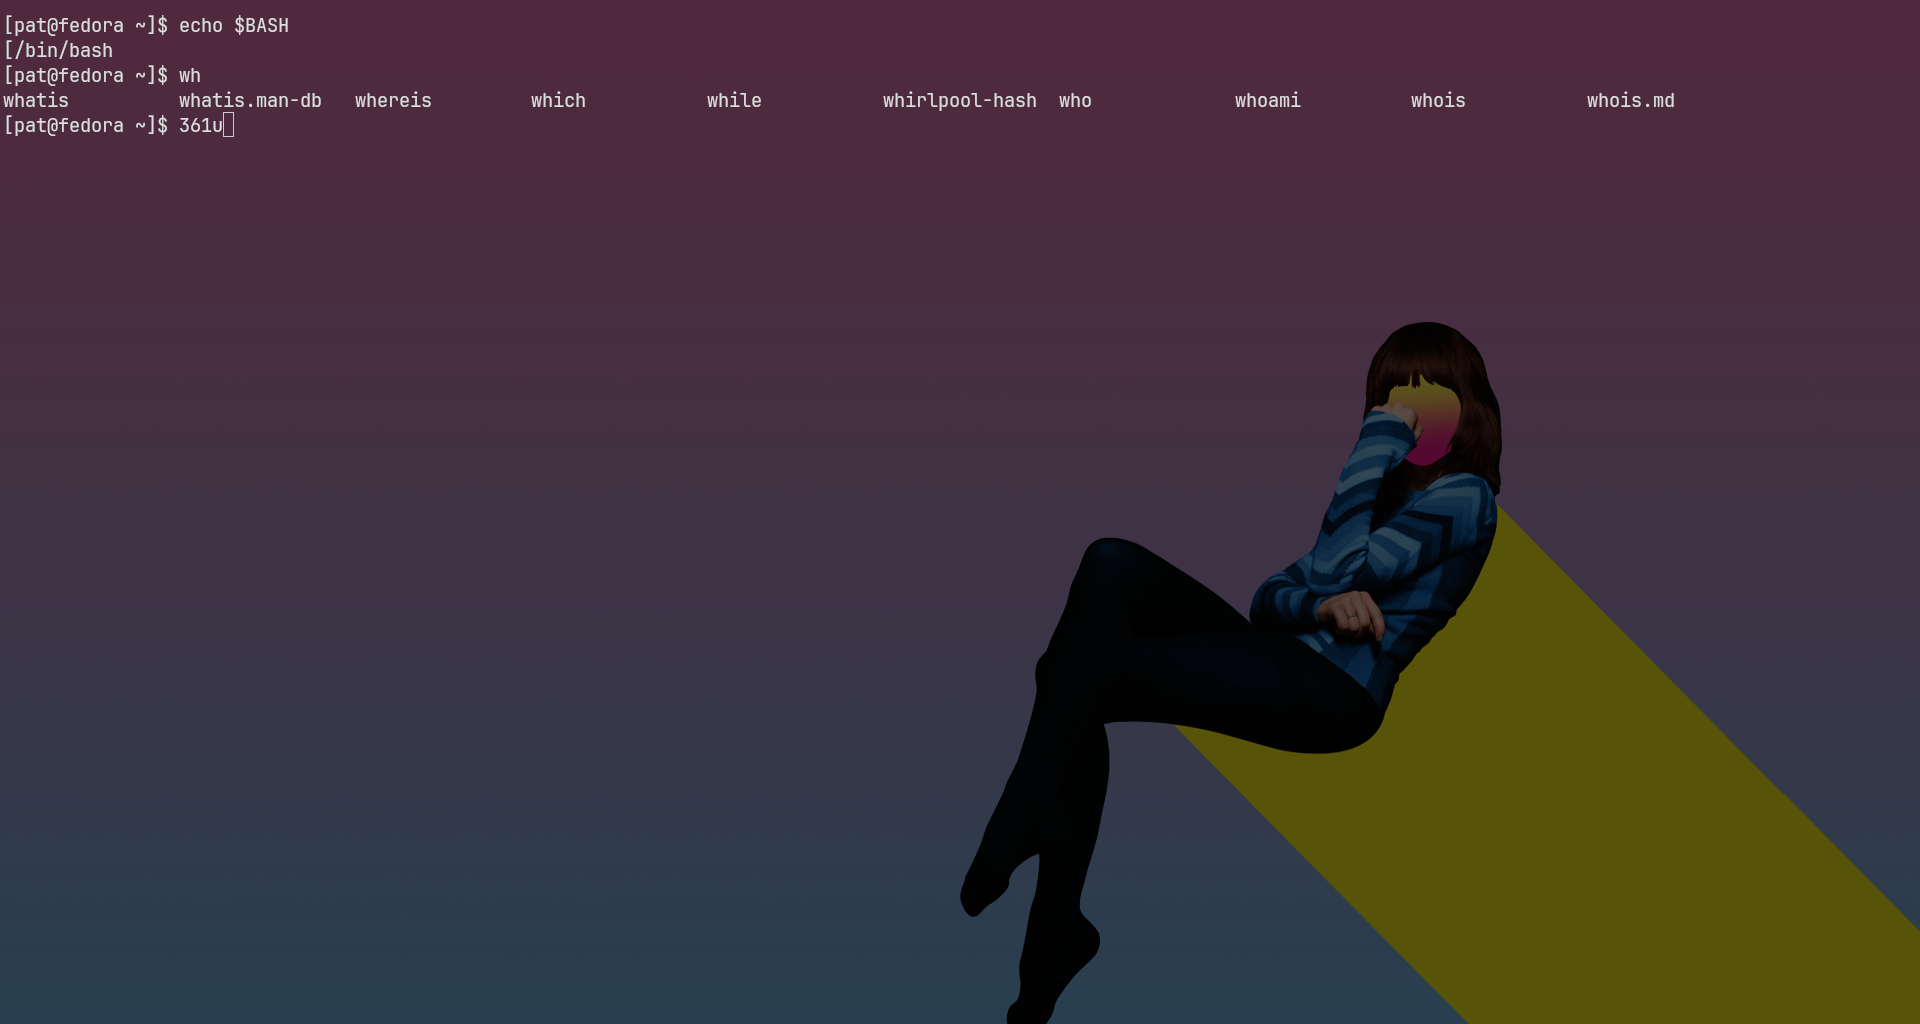
\includegraphics[scale=0.25,trim={0 30cm 0 0},clip]
        {LinuxCapturas/echo-wh.png}
        
\subsubsection{Preguntas Shell}
\begin{enumerate}
    \item ¿Cuáles comandos nos muestran el listado de usuarios activos en el sistema?
    Existen varios comandos pero se suele utilizar users que muestra los nombres de los usuarios, who que adémas imprime la terminal que estan usando, fecha y hora de login y direccion IP o equivalente. Por último está w que imprime los usuarios y sus procesos actuales. 
        \begin{minted}{bash}
        $ users
        $ who
        $ w
        \end{minted}
        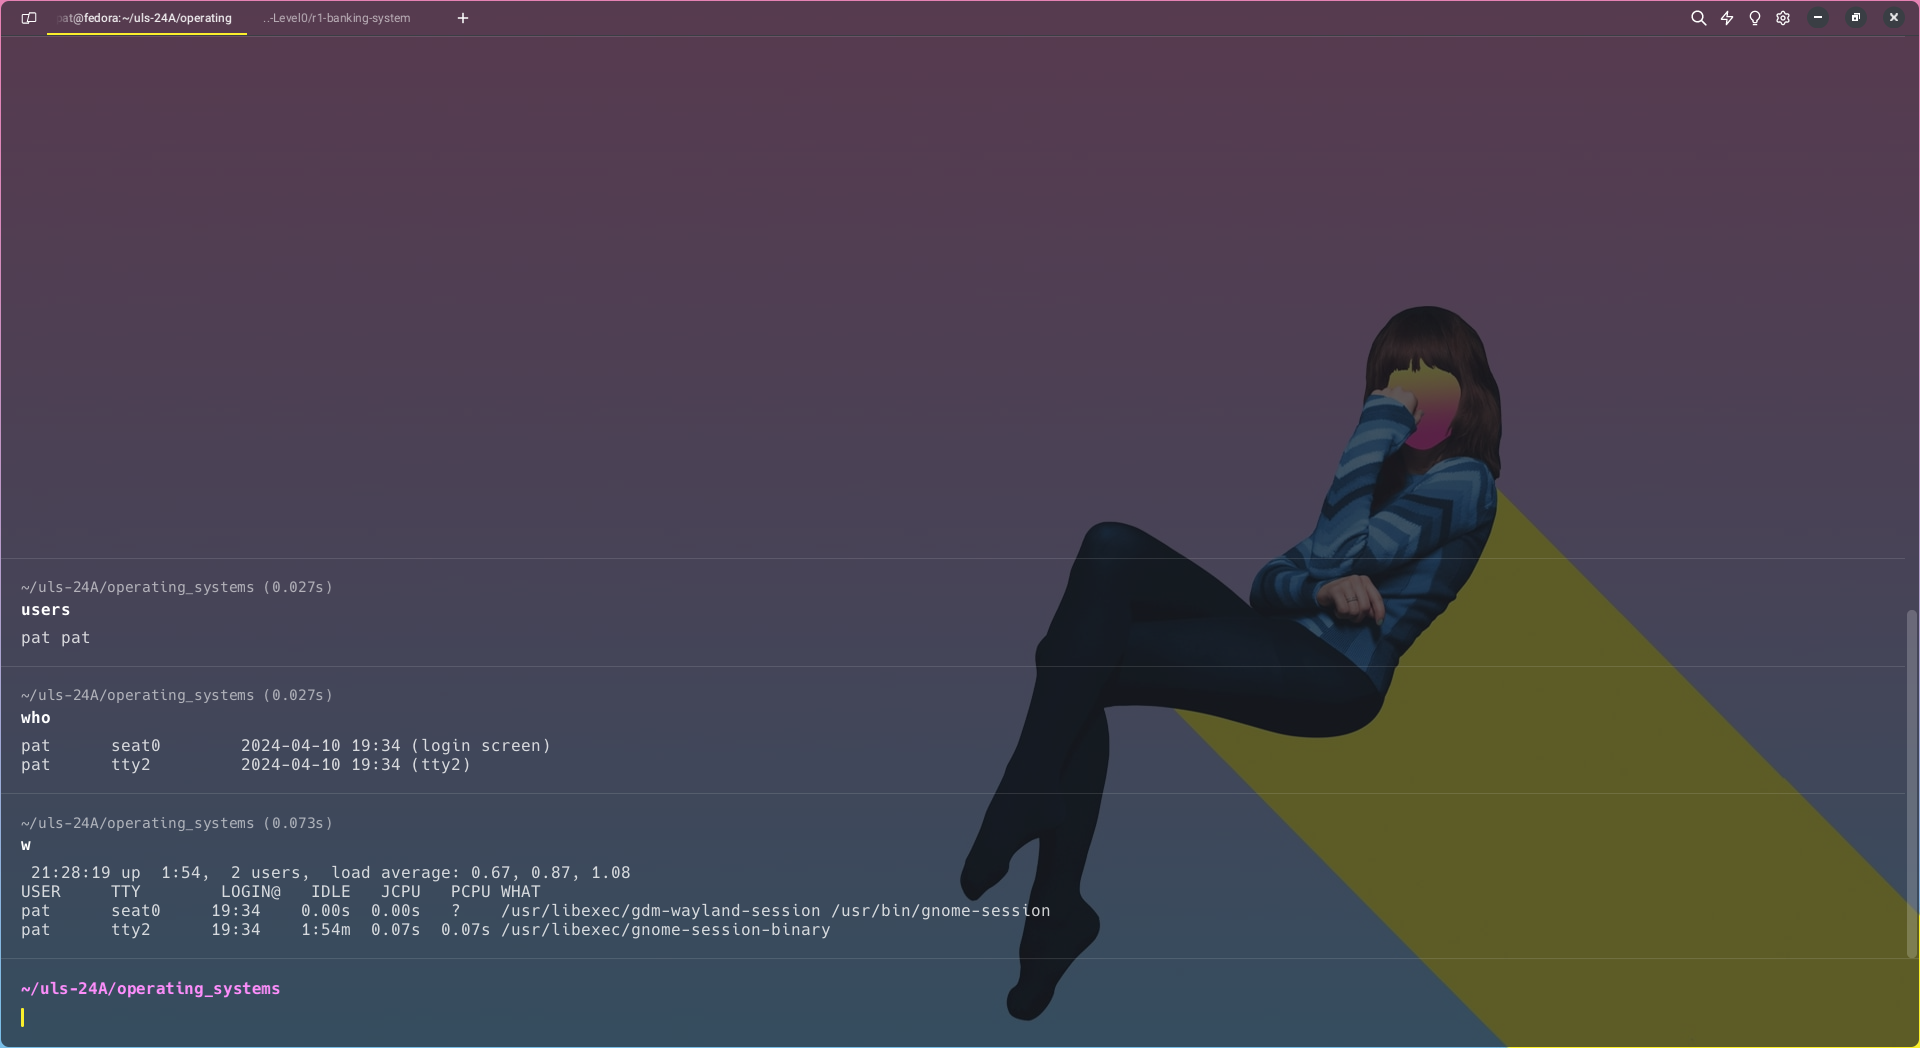
\includegraphics[scale=0.25,trim={0 0 20cm 20cm},clip]{LinuxCapturas/users.png}
        
    \item ¿Cuál sería el comando para desplegar la fecha del último “boot” (Reinicio) del sistema? Si el comando requiere determinadas opciones, inclúyelas. Para mostrar toda la lista de usuarios se usa last reboot y para mostrar solo el ultimo se usa una pipe para llamar head y -1 para mostrar solo 1 elemento desde el final de la lista
    
        \begin{minted}{bash}
        $ last reboot
        $ last reboot | head -1
        \end{minted}
        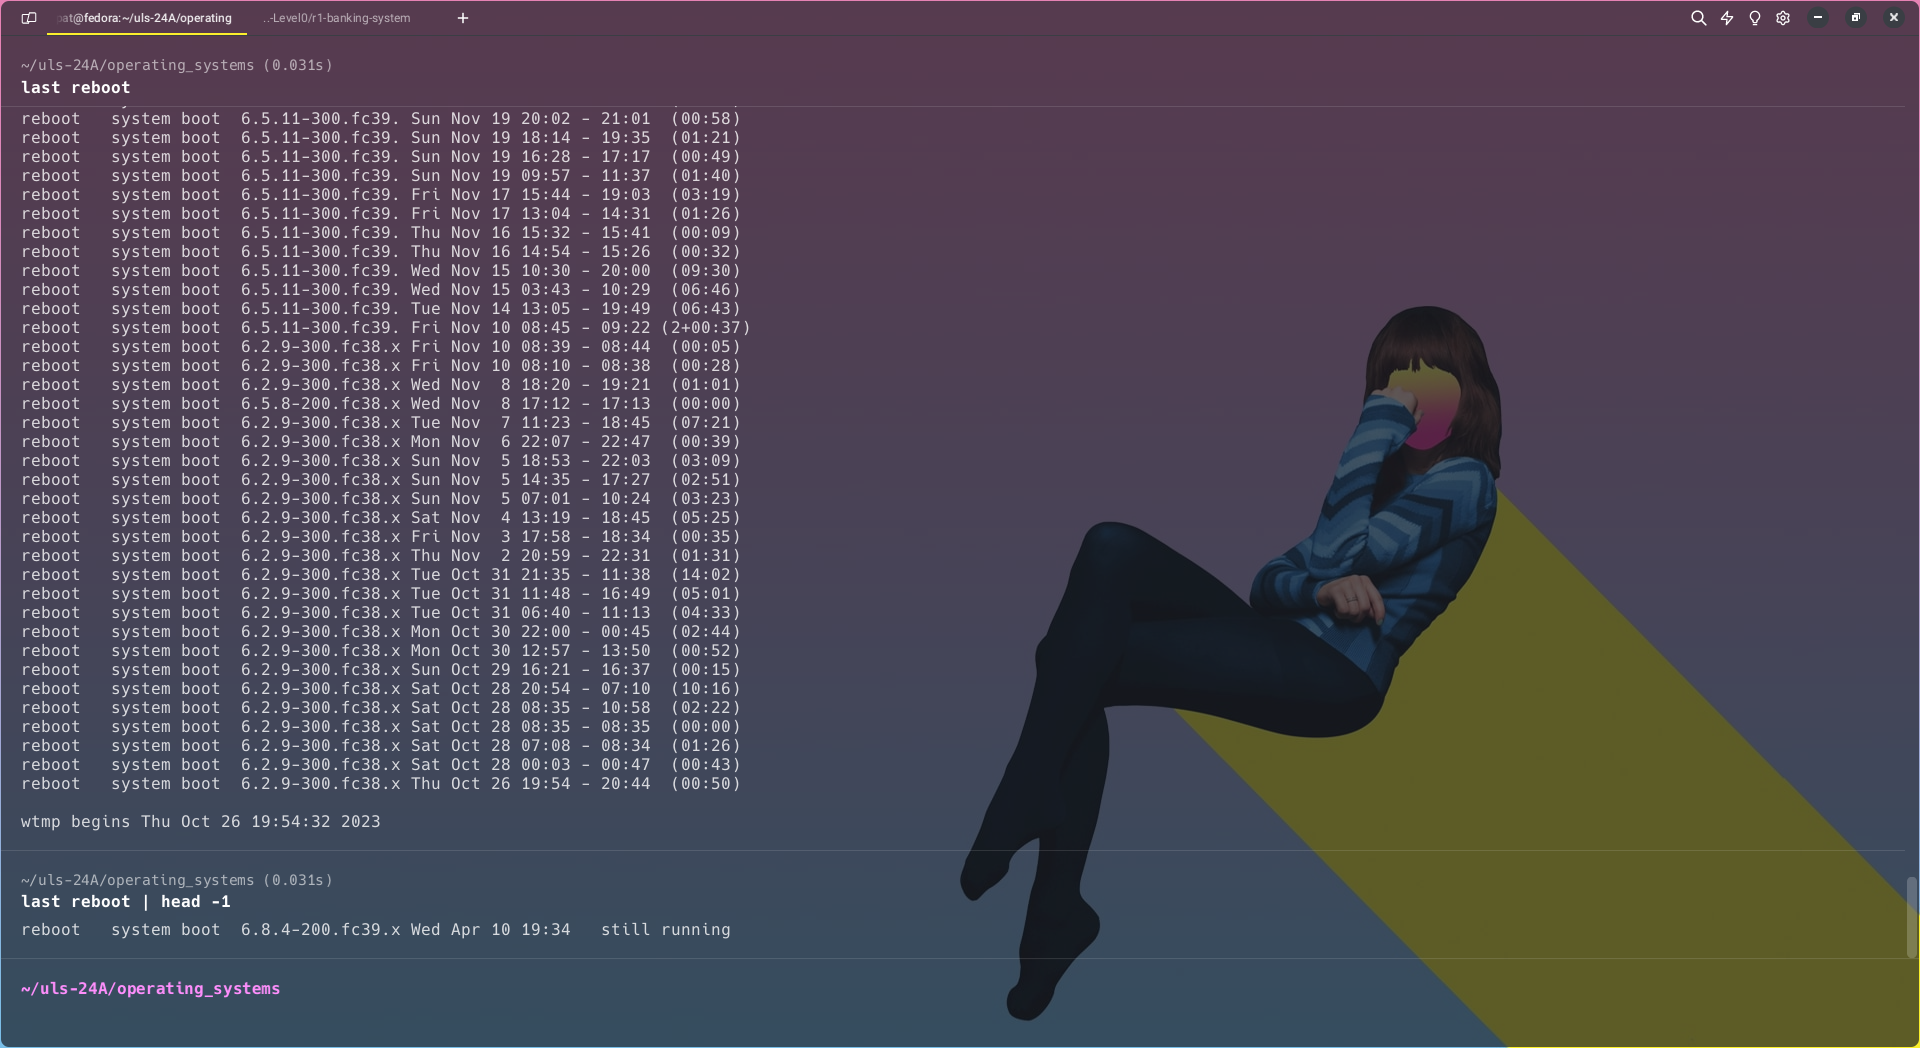
\includegraphics[scale=0.25,trim={0 0 20cm 0},clip]{LinuxCapturas/last-boot.png}  
    
    \item Si un archivo tuviese exclusivamente 3 líneas de texto, ¿cuál sería la diferencia de utilizar los comandos head, tail, more y cat?

    \begin{itemize}
        \item head: Muestra las primeras líneas de un archivo. En este caso, como el archivo solo tiene 3 líneas, mostraría todas ellas.
        \item tail: Muestra las últimas líneas de un archivo. Al igual que head mostraría las 3 líneas.
        \item more: Permite ver el contenido de un archivo página por página. En un archivo de 3 líneas, mostraría todo el contenido a la vez, ya que no hay suficientes líneas para llenar más de una página.
        \item cat: Concatena y muestra todo el contenido de un archivo. En este caso, mostraría las 3 líneas.
    \end{itemize}

    \item Si queremos leer el archivo /etc/passwd (el cual contiene el listado de usuarios del sistema) ¿Cuál sería el más apropiado entre los comandos head, tail, more y cat?¿Por qué?
    \\
    Depende de lo que desee saber el usuario, pero cat debería ser el mas útil puesto que usualmente se quiere saber todos los usuarios y se puede mostrar con facilidad.
    
    \item ¿Cuál es el comando que se recomienda utilizar en lugar de more?
    \\
    Se utiliza el comando less porque permite navegar hacia atrás en el archivo, además de hacia adelante. Esto lo hace más versátil para la visualización de archivos largos o la inspección de logs.

\end{enumerate}
\newpage
\subsubsection{Preguntas Direccionamiento}
Supongamos que nuestro usuario de nombre “fulano” tiene la estructura en su directorio “/home” - obtenida mediante el comando tree - de la siguiente forma: \\
\\ 
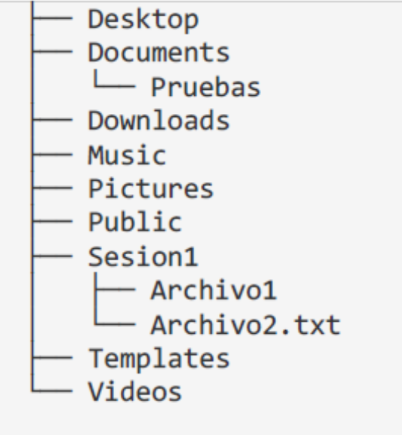
\includegraphics[scale=0.25]{LinuxCapturas/ejercicio.png}

\begin{enumerate}
    \item ¿Qué diferencia existe entre Archivo1 y Archivo2.txt? (pista: En linux las “extensiones” como .txt no indican el tipo de archivo, solo se utilizan como convenciones):
    En Linux las extensiones de archivos solo se utilizan por convención ya que Linux utiliza el contenido y los permisos del archivo para manejarlo. Por ende la diferencia solo radica en el nombre, al menos en lo que concierne al sistema operativo. Esto puede ser comprobado con el comando ls -l en un archivo de ejemplo de Rust:
    \\
    \\ 
    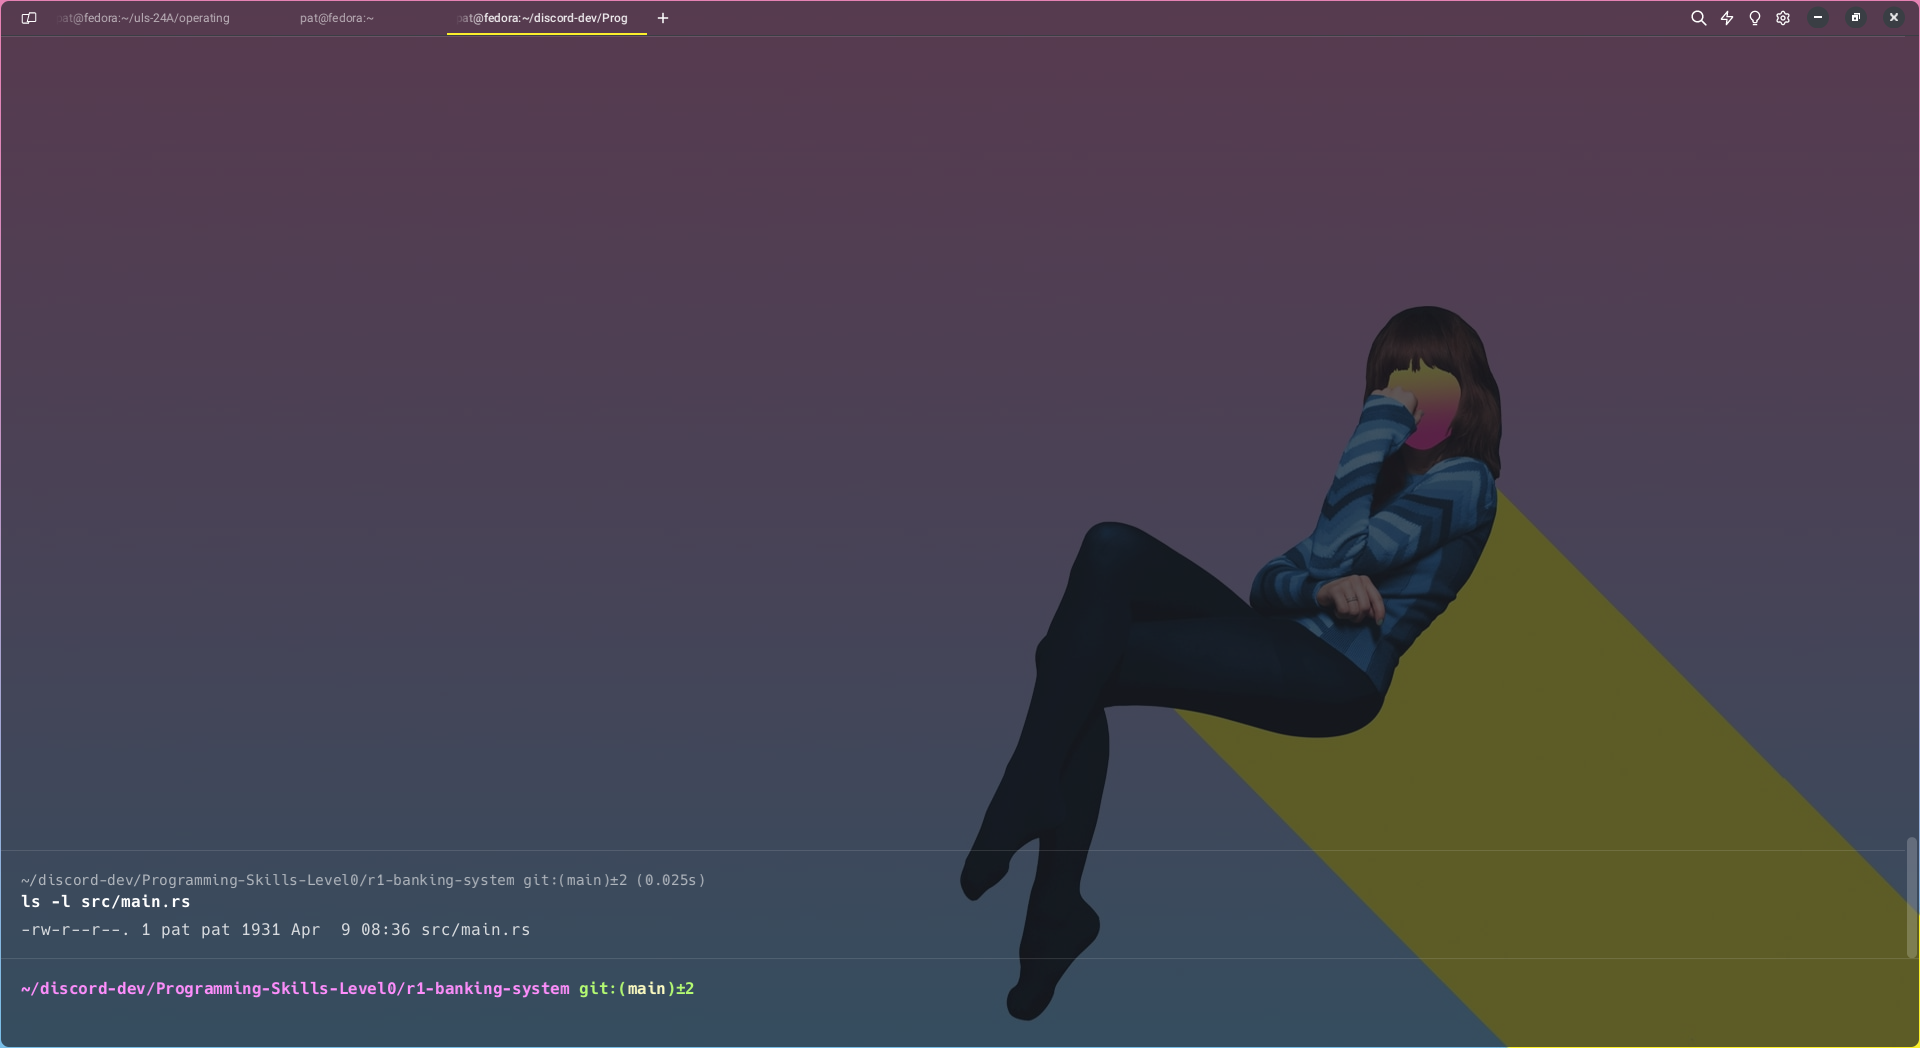
\includegraphics[scale=0.25,trim={0 0 20cm 30cm},clip]{LinuxCapturas/permisos.png}
    
    \item Si la línea en bash aparece como (prompt) : fulano@host: /etc\$. ¿Cuál es el comando para desplegar todo el contenido de Archivo2.txt utilizando direccionamiento relativo al directorio en el que nos encontramos? Si el comando requiere determinadas opciones, inclúyelas
    
    \begin{minted}{bash}
    $ cat ../Sesion1/Archivo2.txt
    \end{minted}

    \item ¿Cuál es el comando para desplegar el contenido del directorio Sesion1, incluyendo los directorios lógicos (también llamados simbólicos) y en orden alfabético, utilizando direccionamiento absoluto (es decir, comenzando por la raíz de todos, “/”)?
    
    \begin{minted}{bash}
    $ ls Sesion1/ -l
    \end{minted}

    \item ¿Cuál es el comando para duplicar la información liberada por tree? 
    Se utilizo -L para manejar la profundidad de los directorios, en este caso solo se utiliza el primer nivel
    
    \begin{minted}{bash}
    $ tree -L 1
    $ tree -L 1 > output.txt
    \end{minted}
    
    \item Valide su respuesta anterior con su propio directorio home, utilizando tanto tree como el comando sugerido por usted.
    
    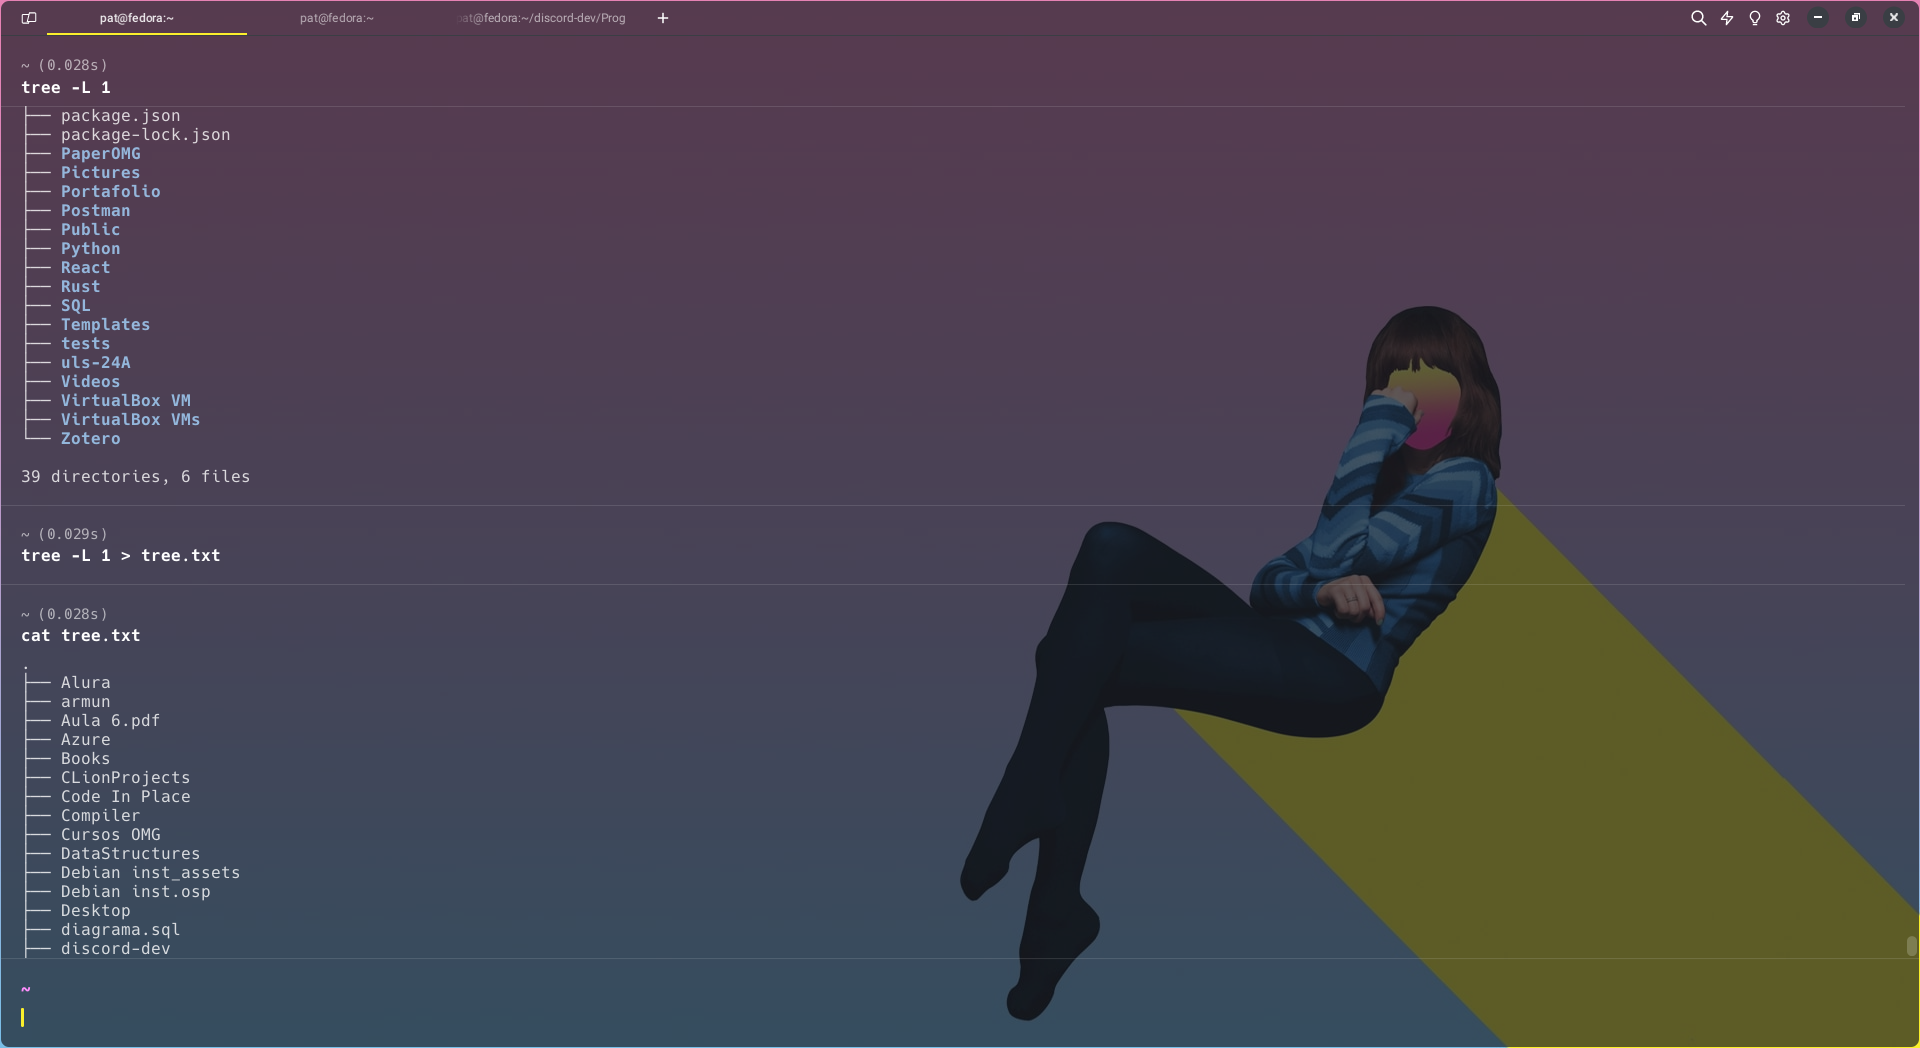
\includegraphics[scale=0.25,trim={0 0 20cm 0},clip]{LinuxCapturas/tree.png} 

\end{enumerate}

\subsection{Manipulando archivos y directorios}
Ejecute los siguientes comandos y conteste las siguientes preguntas:
\begin{minted}{bash}
$ mkdir $HOME/Operativos
$ touch $HOME/Operativos/Arch1
$ touch $HOME/Operativos/Arch2
$ touch $HOME/Operativos/Arch3
\end{minted}

\begin{enumerate}
    \item Comando para copiar el contenido del archivo /etc/passwd a Arch1
    
    \begin{minted}{bash}
    $ cp /etc/passwd Operativos/Arch1
    $ cat Operativos/Arch1
    \end{minted}
    
    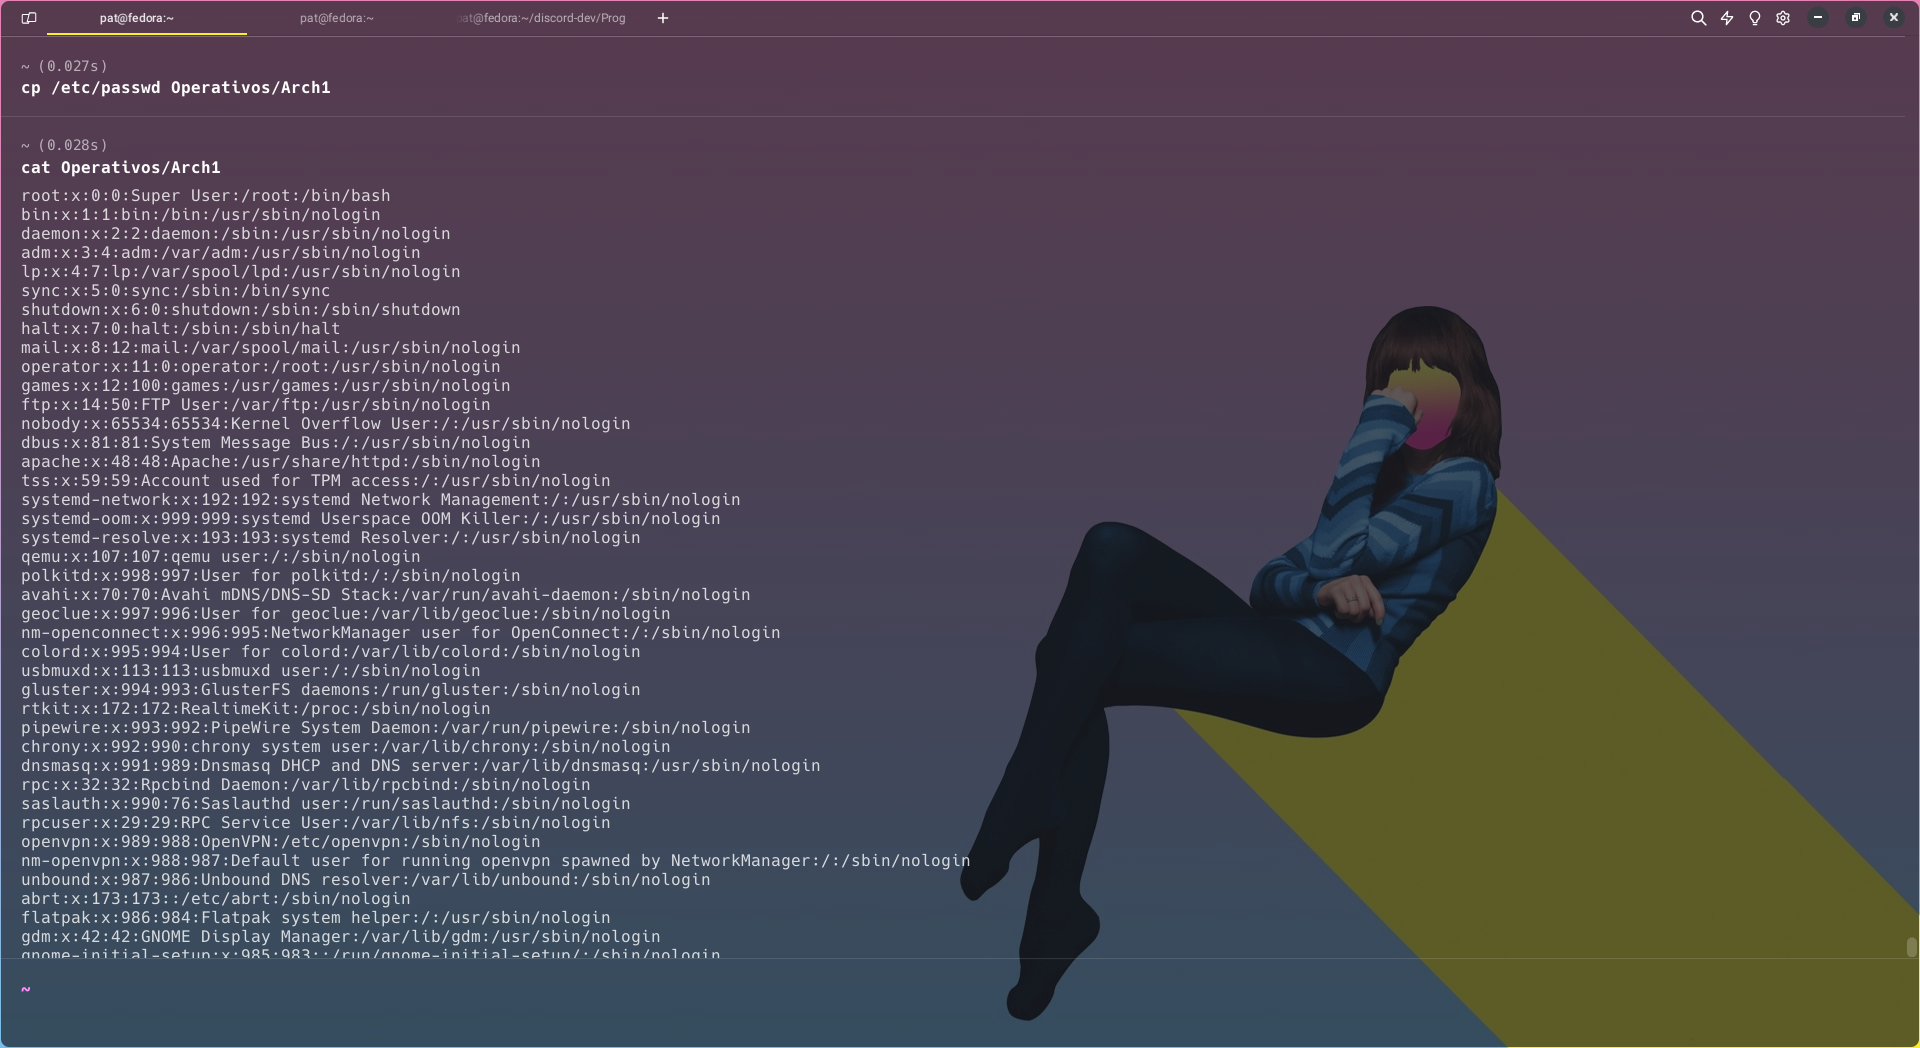
\includegraphics[scale=0.25,trim={0 25cm 20cm 0},clip]{LinuxCapturas/copy.png} 

    \item Comando que copie el archivo Arch1 del paso anterior con el nombre Arch4.

    \begin{minted}{bash}
    # cp crea el archivo de destino si no existe
    $ cp Operativos/Arch1 Operativos/Arch4
    $ cat Operativos/Arch1
    \end{minted}
    
    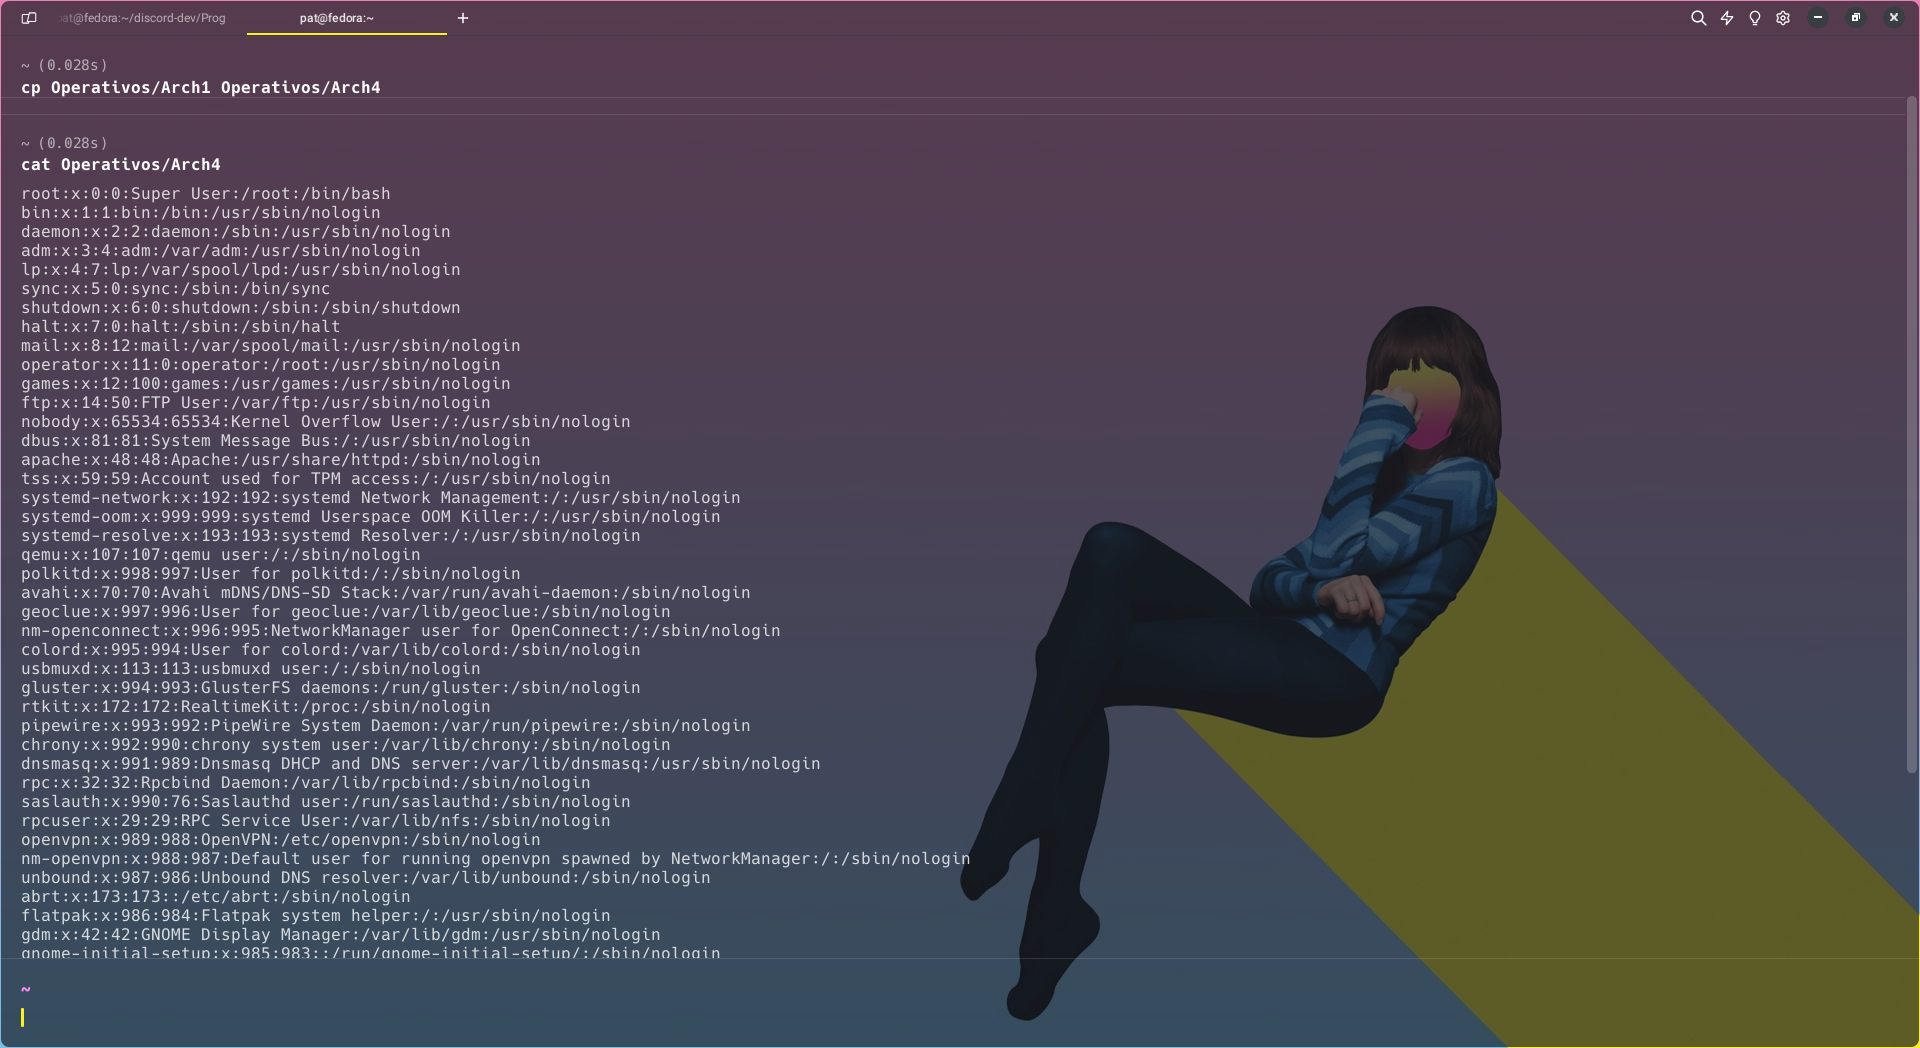
\includegraphics[scale=0.25,trim={0 25cm 20cm 0},clip]{LinuxCapturas/copy2.png} 
    
    \\

    \item Desde \$HOME/Operativos ejecute el comando: mkdir ./Acto1
    \\
    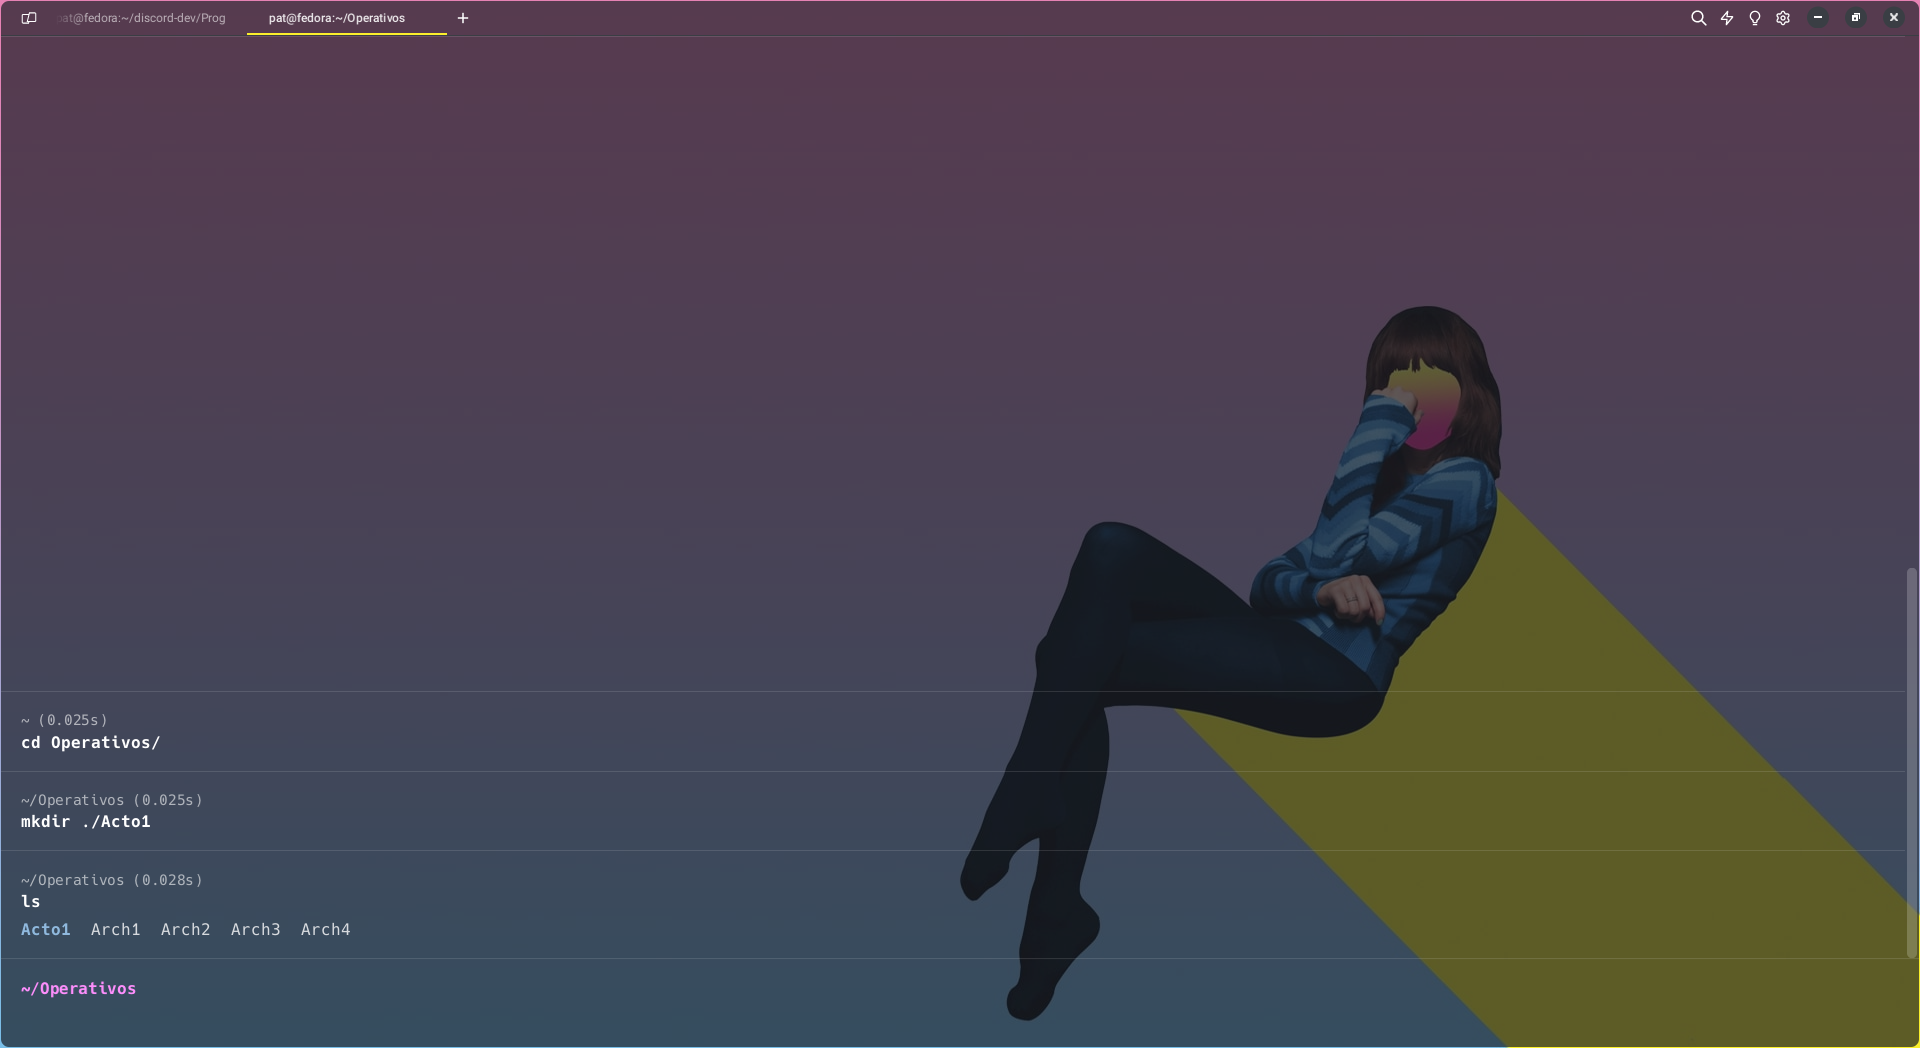
\includegraphics[scale=0.25,trim={0 0 20cm 25cm},clip]{LinuxCapturas/newdir.png} 

    \item Mueva el archivo Arch4 al directorio creado en el paso anterior.
    \begin{minted}{bash}
    $ mv Arch4 Acto1/Arch4
    $ tree
    \end{minted}
    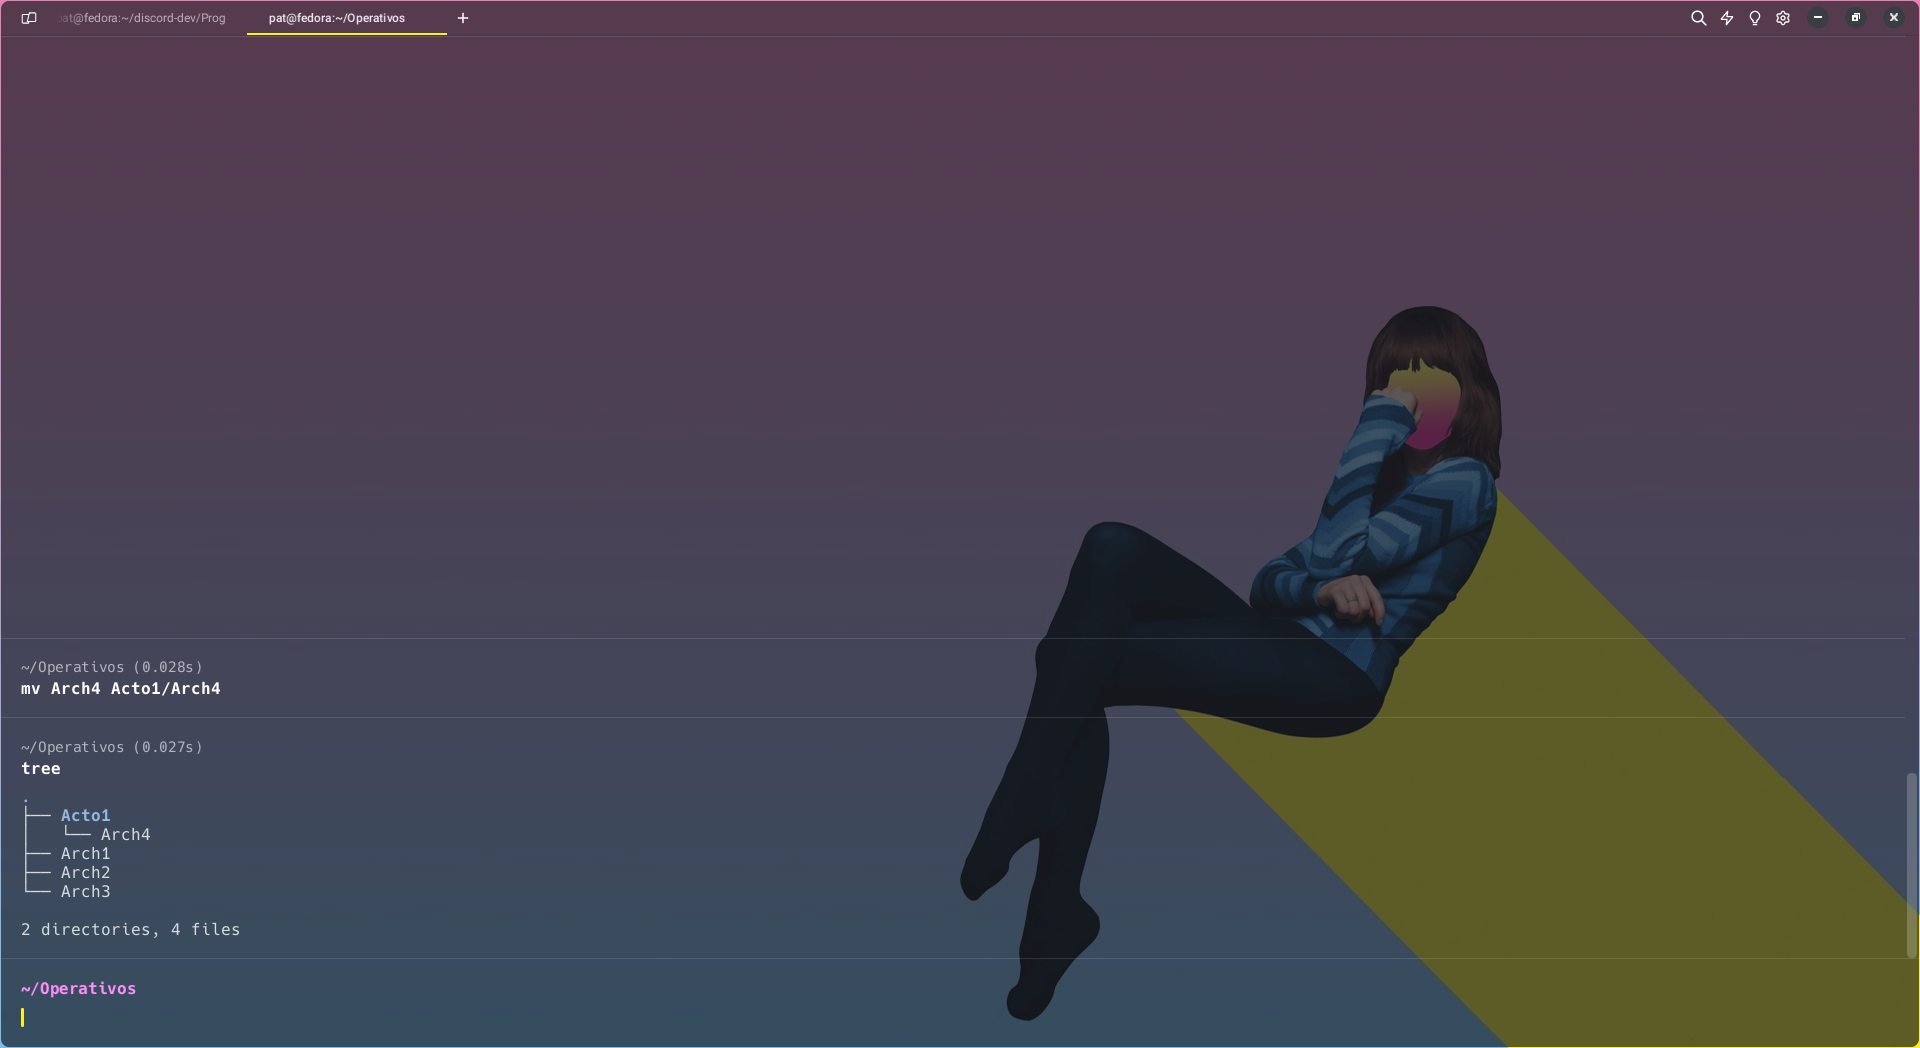
\includegraphics[scale=0.25,trim={0 0 20cm 25cm},clip]{LinuxCapturas/move.png}  

    \item Despliegue la primera línea de Arch4 con direccionamiento absoluto
    \begin{minted}{bash}
    # Se pasa el retorno de cat a head para que solo imprima 1 linea
    $ cat Acto1/Arch4 | head -1
    \end{minted}
    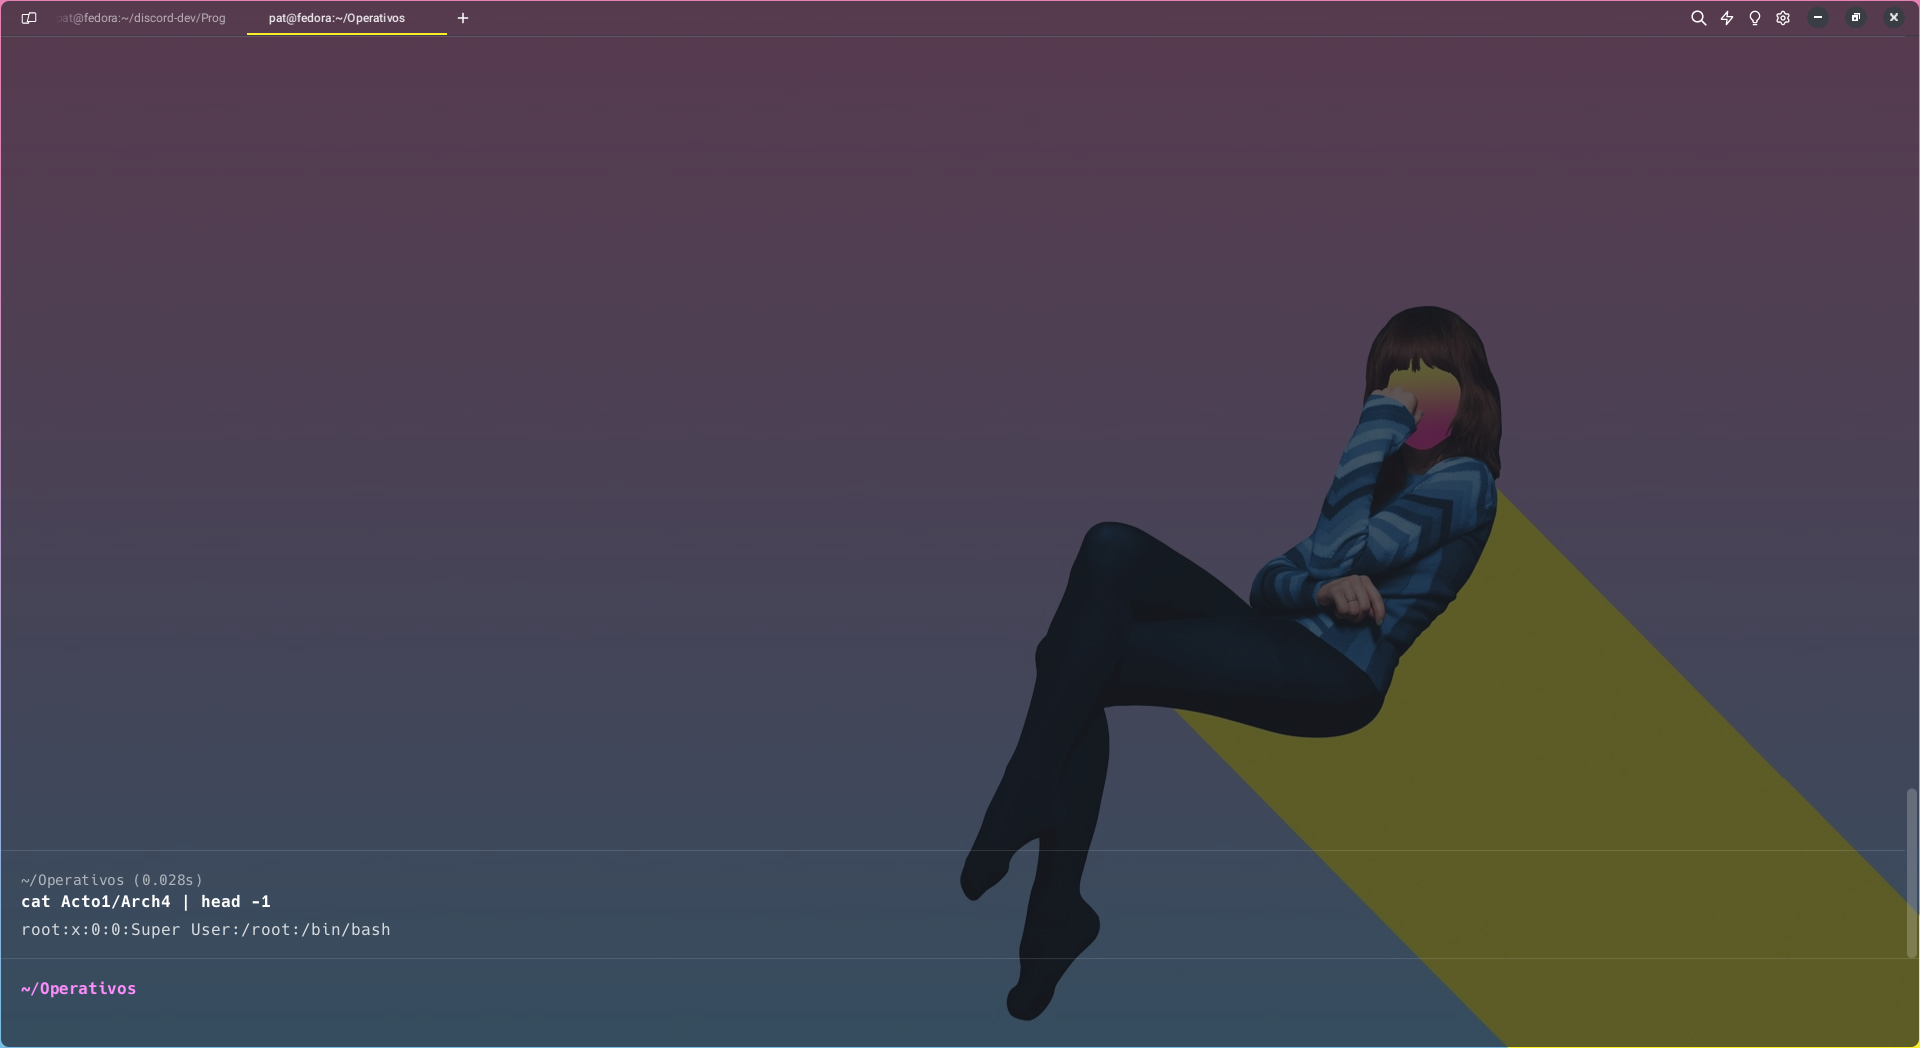
\includegraphics[scale=0.25,trim={0 0 20cm 25cm},clip]{LinuxCapturas/catline.png}

    \item Utilice solamente un único comando para borrar todo el contenido del directorio Operativos
    \begin{minted}{bash}
    # Se utiliza rm con -r para recursivo y -f para evitar archivos protegidos
    $ rm -rf ~/Operativos/
    \end{minted}
    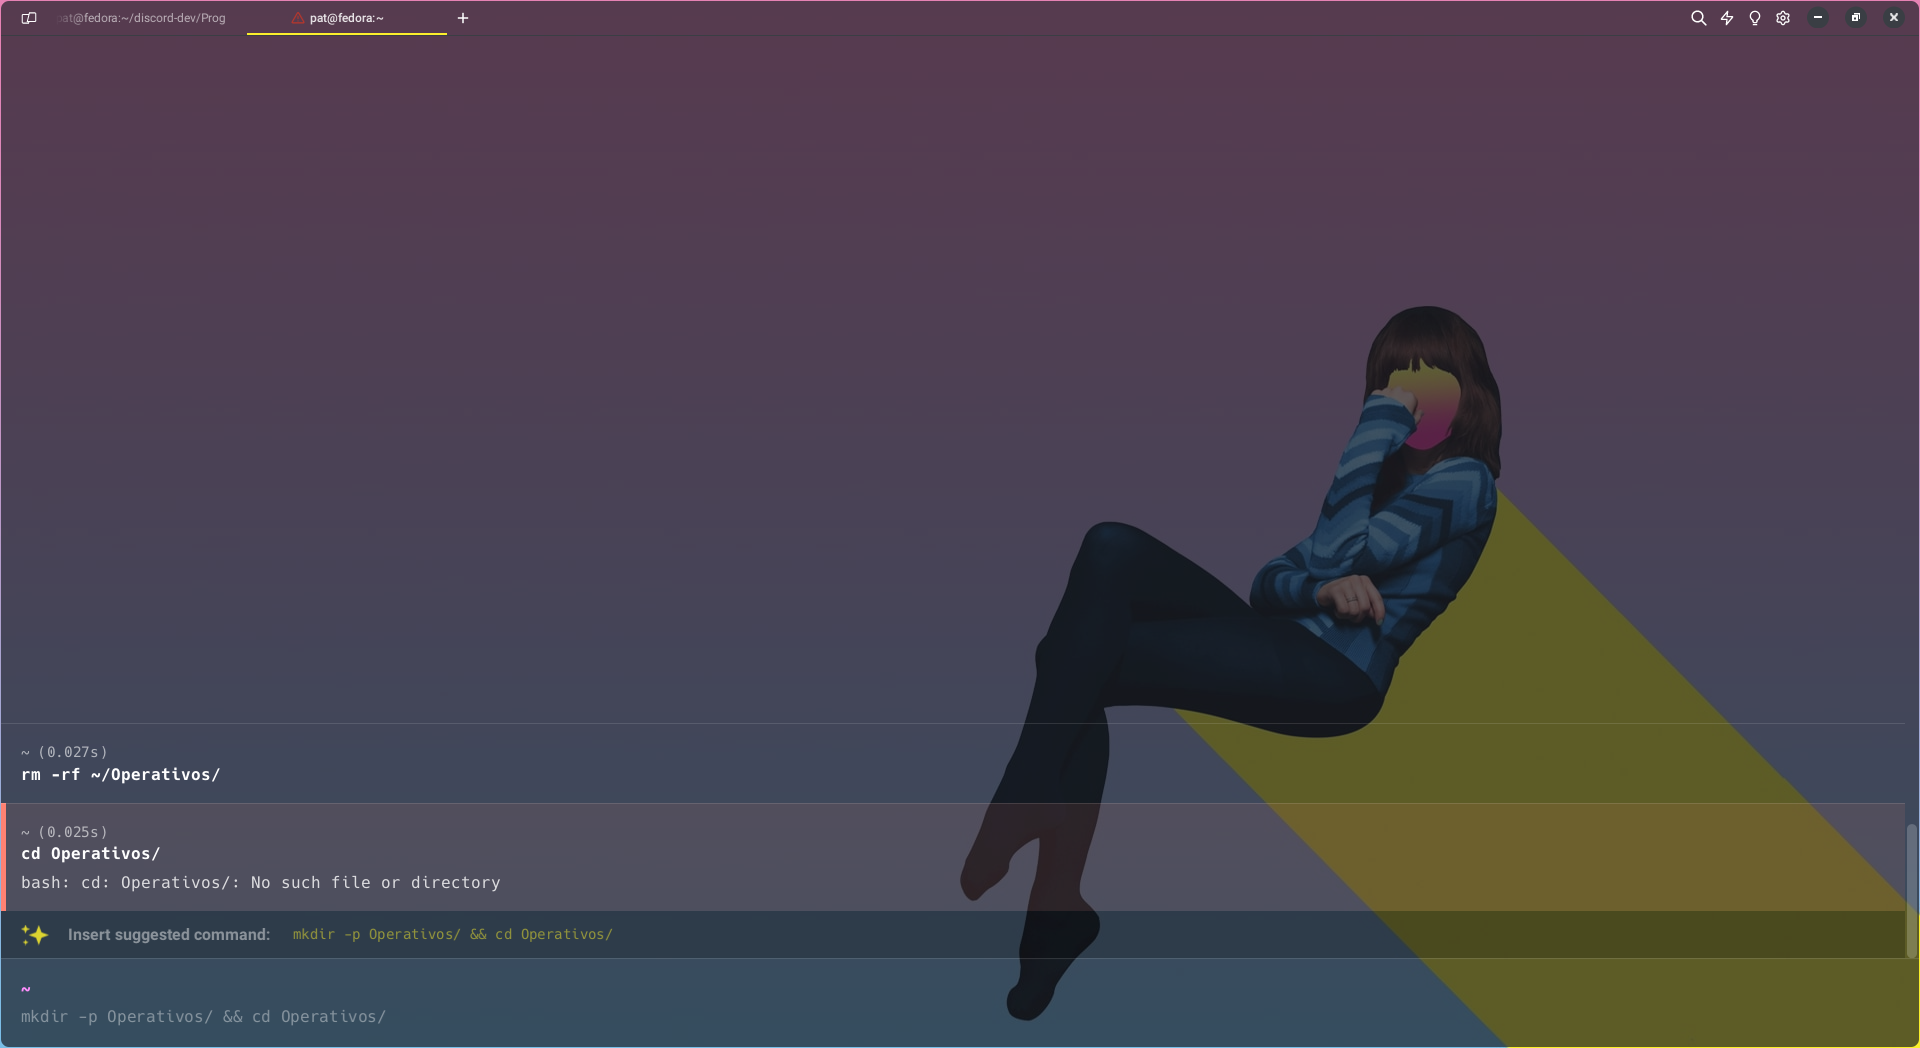
\includegraphics[scale=0.25,trim={0 0 20cm 25cm},clip]{LinuxCapturas/remove.png}

\end{enumerate}

\section{Conclusiones}
\begin{itemize}
    \item Se observa que tanto Windows como Linux ofrecen una gama de comandos para la gestión de archivos y directorios. Por ejemplo, en Windows se utilizan comandos como MD, CD, DIR, y TYPE, mientras que en Linux, comandos como echo, users, who, y w son esenciales para la interacción con el sistema.
    \item La creación y manipulación de carpetas en Windows parece ser intuitiva con comandos simples. En contraste, Linux brinda una mayor flexibilidad y potencia a través de su shell, lo cual puede resultar más atractivo para usuarios con experiencia.
    \item Se nota que en Linux, particularmente en distribuciones como Debian o Arch, hay múltiples métodos para instalar programas, ya sea a través de la terminal o utilizando instaladores como snap, proporcionando así una gran versatilidad1.
\end{itemize}
	%\clearpage
	%\bibliographystyle{apalike}
	%\bibliographystyle{IEEEtranN}
	%\bibliography{bibliography}
\section{Recomendaciones}
\begin{itemize}
    \item Es importante familiarizarse con los comandos básicos de Windows y Linux que se presentan, como MD, CD, DIR, TYPE, COPY, REN, DEL, RD y el uso de la terminal y el shell.
    \item Realizar búsquedas de documentacion de comandos Linux en manpages es bastante útil y práctico
    \item Las flags de los comandos en Linux pueden concatenarse y lograr efectos mas complejos.
    \item Windows también puede manejarse desde la terminal y aprender los comandos de antemano puede ser beneficioso.
\end{itemize}
	
\end{document}
